%----------createLiteral----------------------------------------
\op
{createLiteral}
{creates a new literal}
{createLiteral(Package selectedEObject, String nameValue)}
{The package providing the container for the newly created literal.}
{
\begin{itemize}
 \item nameValue/newName: The name of the newly created literal
 \item idValue/newID: The id of the newly created literal
\end{itemize}
}
{There is no literal whose name equals the parameter-value of 'newID' (see
\ref{subsec:checkOtherNames})}
{The name and the id will be set via input data.}
\begin{figure}[H]
  \centering
  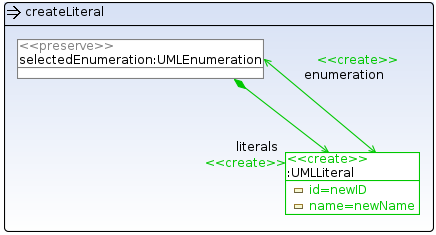
\includegraphics[width=0.65\textwidth]{pics/createLiteral.png}
  \caption{createLiteral}
  \label{createLiteral}
\end{figure}
%----------deleteLiteral----------------------------------------
\op
{deleteLiteral}
{Deletes a literal}
{deleteLiteral(Literal selectedEObject)}
{The literal which should be deleted}
{-}
{-}
{For a better readability this is a simplified version of the
'deleteLiteral'-transformation and will only cover cases where the
literal has no references to other elements. Such a
complex transformation rule exits but won't be listed here.}
\begin{figure}[H]
  \centering
  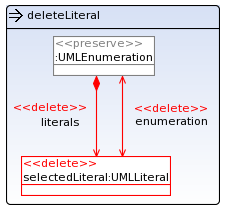
\includegraphics[width=0.4\textwidth]{pics/deleteLiteral_emptyAndUnreferenced.png}
  \caption{deleteLiteral}
  \label{deleteLiteral}
\end{figure}
%----------editLiteralName----------------------------------------
\op
{editLiteralName}
{edits the name of a literal}
{editLiteralName(Literal selectedEObject, String nameValue)}
{The literal whose name should be renamed.}
{
\begin{itemize}
 \item nameValue/newName: The new name
\end{itemize}
}
{There is no literal in the same package whose name equals the parameter-value of
'newName' (see
\ref{subsec:checkOtherNames})}
{The \textless\textless create\textgreater\textgreater  -symbol in the image
means that even if the attribute exists its value will be overwritten.
'newName' is the placeholder for the input name.}
\begin{figure}[H]
  \centering
  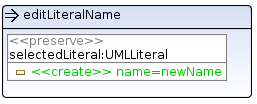
\includegraphics[width=0.4\textwidth]{pics/editLiteralName.png}
  \caption{editLiteralName}
  \label{editLiteralName}
\end{figure}
%----------moveLiteral----------------------------------------
\op
{moveLiteral}
{moves a literal from an enumeration to another}
{moveLiteral(Literal selectedEObject, Enumeration tgt)}
{The literal which should be moved.}
{
\begin{itemize}
 \item tgt/tgt[moveLiteral]: the target enumeration
\end{itemize}
}
{There is no literal with the same name in the target context (see
\ref{subsec:checkOtherNames})}
{Only references will change.}
\begin{figure}[H]
  \centering
  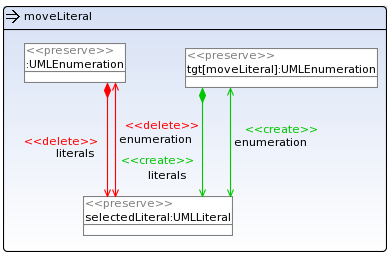
\includegraphics[width=0.65\textwidth]{pics/moveLiteral.png}
  \caption{moveLiteral}
  \label{moveLiteral}
\end{figure}